\documentclass{article}
\usepackage{fullpage}
%%%%%%%%%%%%%%%%%%%%%%%%%%%%%%%%%%%
\usepackage{graphicx}
\usepackage{epstopdf}
\usepackage{amsthm}
\usepackage{amsmath}
\usepackage{amssymb}
\usepackage{caption}
\usepackage{subcaption}
\usepackage[all]{xy}



\everymath{\displaystyle}

\newenvironment{solution}
  {\begin{proof}[Solution]}
  {\end{proof}}
\newtheorem{definition}{Definition}
\newtheorem{example}{Example}
\newtheorem{theorem}{Theorem}
\newtheorem{remark}{Remark}
\newtheorem{lemma}{Lemma}
\newtheorem{inequality}{Inequality}
\newtheorem{proposition}{Proposition}

\providecommand{\abs}[1]{\left|#1\right|}
\providecommand{\norm}[1]{\lVert#1\rVert}
%%%%%%%%%%%%%%%%%%%%%%%%%%%%%%%%%%%
\begin{document}
\title{AMATH574 Conservation Laws and Finite Volume Methods\\ Winter Quarter 2015\\ Project Draft: F-wave method for nonlinear equations with spatially varying fluxes.}
\author{Instructor : Professor Randall Leveque\\ Student: Hai Zhu(zhuh1106@uw.edu), Xin Yang (yangxin@uw.edu)\\ Due date: Wednesday, Feb. 18, 2015}
%\date
\maketitle

\section{Abstract}
We study the f-wave method for elastic waves in heterogeneous media.
\section{Introduction and Overview}
\subsection{Physical Model}
In this project, we are considering 1D elasticity equations
\begin{align}
\epsilon(x,t)_t-u(x,t)_x=0 \label{strain}\\
\rho(x) u(x,t)_t-\sigma(\epsilon,x)_x=0 \label{n2}
\end{align}
where, $\epsilon$ is the strain, $u$ is the velocity, $\rho$ is the density and $\sigma$ is the stress. These are classical mechanics equations in Lagrangian form. Equation \eqref{strain} comes from the definition of strain. If $v(x)$ is the displacement of small element at $x$, then the strain, i.e. the relative change of displacement is $\epsilon=\frac{dv(x)}{dx}$. Equation \eqref{strain} is then obtained by taking a time derivative. The stress is the force per unit area. Therefore Equation \eqref{n2} is simply Newton's second law. In order to close the system, often the constitutive law $\sigma=\sigma(\epsilon)$ is introduced. The relation depends on the material, for instance:
\begin{itemize}
\item The simplest linear media:
\begin{align}
\sigma(x,t)=K(x)\epsilon(x,t)
\label{lins}
\end{align}
here $K(x)$ is the bulk modulus or Young's modulus which determines the stiffness of the material.
\item Relatively simple nonlinear model with quadratic relation:
\begin{align}
\sigma(x,t)=K(x)\epsilon(x,t)+\beta K^2(x)\epsilon^2
\label{quads}
\end{align}
\item Nonlinear model with quadratic relation:
\begin{align}
\sigma(x,t)=\exp(K(x)\epsilon(x,t))-1
\label{exps}
\end{align}
\item (Periodically) Layered media:
\begin{align}
K(x)=\left\{
\begin{array}{cc}
K_A & \mbox{if }j\delta<x<(j+\alpha)\delta \mbox{ for some integer } j,\\
K_B & \mbox{otherwise.}
\end{array}
\right.
\end{align}
Here $\delta$ is the period and $\alpha$ is the proportion of the first type of medium. 
\end{itemize}
In small $\epsilon$ case, Equation \eqref{exps} is approximated by Equation \eqref{quads} if $\beta=0.5$ while they are both approximated by the linear model in Equation \eqref{lins}.
\subsection{Issues with variable coefficients equations and the idea of f-wave method}
As we have seen in class, the variable coefficients can sometimes be treated as the solution to an additional PDE. For instance, if we assume the linear media for the 1D elasticity equations above. $K(x)_t=0$ could be added to the system. Therefore,
\begin{align*}
\epsilon(x,t)_t-u(x,t)_x=0 \\
\rho(x) u(x,t)_t-(K(x)\epsilon)_x=0 \\
K(x)_t=0
\end{align*}
becomes a nonlinear (linearly degenerate) constant coefficient system of conservation law. This additional equation introduces a new line of characteristics $x=x_{i-1/2}$ which is stationary. As a result of this new discontinuity locating on the edges of cells, if one still work with the original system with one less equation, the decomposition of $Q_i-Q_{i-1}$ using eigenvectors (w-waves) would be wrong without the consideration of the jump across $x_{i-1/2}$. However, notice that in the wave-propagation form updating formula
\begin{align}
Q_i^{n+1}=Q_i^{n}-\frac{\Delta t}{\Delta x}\left[\sum (\lambda^p)^-W_{i+1/2}^p+\sum (\lambda^p)^+ W_{i-1/2}^p\right]
\end{align}
there's no contribution of the wave with speed zero. Therefore, one may seek for different approaches. As can be seen from the name, the idea of f-wave method is to decompose the flux difference $f(Q_i)-f(Q_{i-1})$ using eigenvector of the original system:
\begin{align}
f(Q_i)-f(Q_{i-1})=\sum \beta^p_{i-1/2} r^p_{i-1/2}\equiv \sum Z^p_{i-1/2}.
\end{align}
Since the Rankine-Hugoniot condition across the discontinuity with speed zero means the continuity of the flux, both the wave-propagation formula and the Rankine-Hugoniot condition suggest that considering propagations of discontinuities of the fluxes is more appropriate.
\subsection{Implementation}
The f-wave method uses the updating formula:
\begin{align}
Q_i^{n+1}=Q_i^{n}-\frac{\Delta t}{\Delta x}\left[\sum sign((\lambda^p)^-) Z_{i+1/2}^p+\sum sign((\lambda^p)^+) Z_{i-1/2}^p\right]
\end{align}
Therefore, the change from w-wave to f-wave is simple provided the approximate Riemann solver is given. Hence, we give the following procedure in the construction of the codes for the Riemann solver:
\begin{enumerate}
\item Obtain the approximate Jacobian $A_{i-1/2}$ or, alternatively, get the eigenvalues $s^p$ and eigenvectors $r^p$ of the approximate Jacobian.
\item Decompose the flux difference to get $\beta=R^{-1}(f(Q_i)-f(Q_{i-1}))$. The p-th f-wave is then given by $\beta^p r^p$.
\item Sum up $A^- \Delta q$ all the left-going f-wave, and $A^+ \Delta q$ all the right-going wave. In this problem, since we only have two equations and the sound speed is $\pm_c$, $A^- \Delta q$ contains the 1-f-wave and $A^+ \Delta q$ contains the 2-f-wave.
\item If needed, $W^p=Z^p/s^p$ the w-waves can be recovered by a division. However, numerical error may occur when $s^p$ is close to zero. 
\end{enumerate}
\section{Objective}
\begin{enumerate}
\item Implement the f-wave method for nonlinear elastic waves in heterogeneous media. Reproduce some of the figures in \cite{bale2002} \cite{leveque2003} and \cite{ketcheson2012}.
\item Have a more comprehensive discussion of the f-wave method and problem. Mostly on the verifications of the details of the method mentioned in the paper and textbook. p. 314 $\&$ p. 333 in the textbook. Some aspects include:
    \begin{itemize}
    \item The disadvantages of using cell-edge flux functions in wave-propagation algorithm metioned in \cite[p. 957]{bale2002}
    \item Justification of the Riemann solver used in \cite[p. 967]{bale2002}
    \item The non-conservation when using w-wave in wave-propagation algorithm for 1) nonlinear autonomous systems with simple Riemann solver (HLL? p. 328 in the textbook), 2) non-autonomous systems with "Roe average" Rieman solver.
%    \item The non-conservation when using w-wave in wave-propagation algorithm and possible fix approximate Riemann solvers for 1) nonlinear autonomous systems with simple Riemann solver (HLL? p. 328 in the textbook), 2) non-autonomous systems with "Roe average" Rieman solver. p. 318 in the textbook
    \item The slight difference of using $\mathcal{Z}=s\mathcal{W}$ in the limiter to get high-resolution methods. \cite[p. 964]{bale2002} p. 335 in the textbook.
    \item The new line of discontinuities caused by the discontinuities of the coefficient. \cite[p. 960]{bale2002}
    \item The breakdown of f-wave method in the case of singular flux (delta distribution).  \cite[p. 961]{bale2002}
    \end{itemize}
\item If possible, have some discussion on the dispersive properties of layered media i.e, solitons and shocks.
\end{enumerate}
The importance of the goals is decreasing in the order.
\section{Theoretical Background}


\section{Computational Results}
\begin{figure}
  \centering
  % Requires \usepackage{graphicx}
  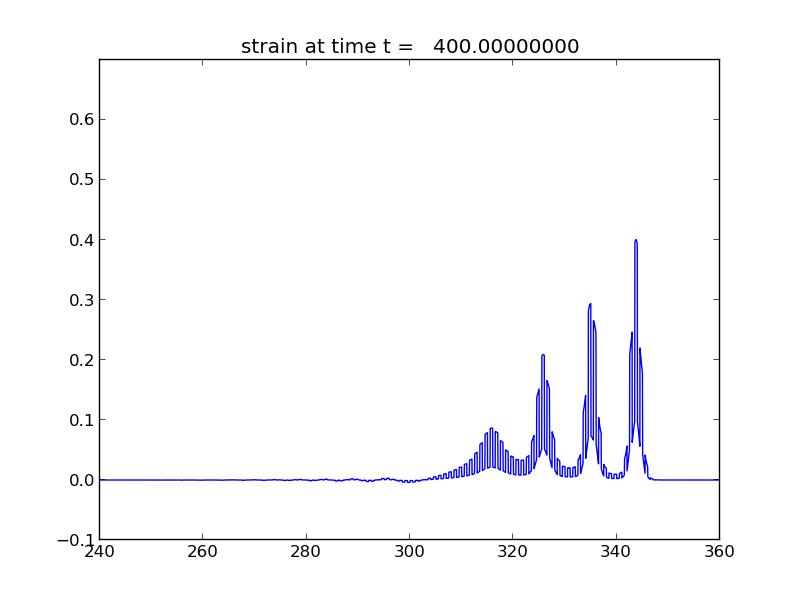
\includegraphics[width=\textwidth]{frame0040fig1.png}\\
  \caption{Stegoton!}\label{stegoton}
\end{figure}


\section{Summary and Conclusions}



%\section{Appendix A: MATLAB functions used and brief implementation explanation}
%\section{Appendix B: MATLAB codes}
%\section{Appendix C(optional)} Any algebraically intense calculations.

\begin{thebibliography}{9}
\bibitem{bale2002}
D. S. Bale, R. J. LeVeque, S. Mitran, and J. A. Rossmanith, SIAM J. Sci. Comput 24 (2002), 955-978.
\bibitem{leveque2003}
Randall J. LeVeque and Darryl H. Yong, SIAM J. Appl. Math., 63 (2003), pp. 1539-1560.
\bibitem{ketcheson2012}
David I Ketcheson, Randall J. LeVeque Comm. Math. Sci. 10 (2012), pp. 859-874.
\end{thebibliography}

\end{document}
